\chapter{Preliminary Evaluation}\label{ch:prelim_eval}

Fine grained modularity in I/O systems, exhibited in the sDDF design, has the
potential to degrade performance because of the extra number of context switches involved.
Before embarking on the remainder of this thesis, we can already demonstrate that such a
design is feasible for simple high performance I/O systems.

\section{Evaluation setup}
The sDDF currently supports a minimal networking-focused system capable of echoing Ethernet packets it receives. It
runs on a single core of a Freescale i.MX 8M Mini quad applications processor with 2Gb RAM, running at 1.2 GHz with a 1Gbps NIC.
The test system comprises of the following 5 PDs:
\begin{enumerate}
\item Ethernet Driver: a minimal driver based on \ref{s:driver_model}.
\item Rx Mux: a minimal receive path multiplexer that reads the Ethernet header and compares the
destination MAC address as per \ref{s:mux_design}.
The multiplexer was developed to support one client only and does not contain any policy logic. 
\item Tx Mux: a minimal transmit path multiplexer as per \ref{s:mux_design} that supports a single
client. Similarly, it also does not contain any policy logic.
\item Copy Component: a component that copies data from the shared data region to the client's own address space. 
\item Client: an echo server. The client uses lwIP \cite{Dunkels_01} as an IP stack library to process incoming 
UDP packets and simply send them back unmodified. 
\end{enumerate}

We use ipbench \cite{Wienand_Macpherson_04} as a distributed load generator to send 1472byte sized UDP packets to test the seL4 based system. 
ipbench runs on a 4-node x86 cluster and counts the number of successful replies from the target system to measure the achieved throughput and latencies.

We compare the seL4 based system against a Linux system (version 6.1.1) on the same hardware. We use a simple user level application which 
reads and then writes all packets immediately back using sockets as described in \ref{s:sockets}. 
In order to determine the CPU utilisation of both systems, we run an idle thread at low priority to count the number of idle cycles. 

\section{Results}

\begin{figure}[h]
    \centering
    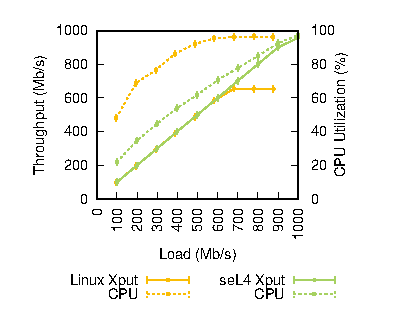
\includegraphics[width=12cm]{5comp.eps}
    \caption{Linux vs seL4 Networking Performance}
    \label{f:perf}
\end{figure}

\autoref{f:perf} compares the performance (achieved throughput and CPU utilisation over applied load) of both systems. 
We can see that the sDDF based system's throughput scales with applied load and manages to saturate the wire, while
Linux scales linearly to about 650 Mb/s and then plateaus. When comparing the CPU utilisation of both systems, we
can see that the reason behind this plateau in throughput is because Linux uses significantly more CPU cycles 
to handle a given load than the sDDF based system. Furthermore, the CPU utilisation of the sDDF system also scales 
sub-linearly with increasing load which indicates efficient batching.

\begin{figure}[h]
    \centering
    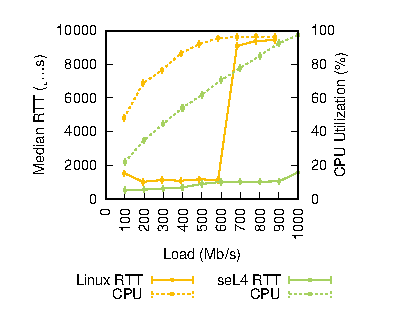
\includegraphics[width=12cm]{latency.eps}
    \caption{Linux vs seL4 Networking Latencies}
    \label{f:perf_latencies}
\end{figure}

\autoref{f:perf_latencies} compares the round trip time (RTT) latency and CPU utilisation over applied load of both systems. The latency measured
is the median result taken from a sample size of 200,000 packets. We can see that the sDDF demonstrates a much faster round trip time over Linux, 
and, unlike Linux, the round trip time does not blow up as the system becomes saturated. 

\section{Current Limitations}
The above results demonstrate that a simple, componentised networking system on seL4 can achieve higher throughput and lower latencies than a typical
networking system on a monolithic kernel. However, the current prototype does not currently support multiple client applications and 
is limited to single core systems. As such, the multiplexer components are very simple and do not contain any policies. Furthermore, the 
preliminary evaluation is limited as it only tests a system with symmetric traffic on the receive and transmit paths. In a real
networking system, this would not be the case. For example, a web server would have much higher throughput on the transmit path than the receive path.
Finally, the above evaluation was limited to running on a single core only which is not the typical set up for high throughput networking systems.
% TODO: Add other stuff that is currently unsupported: eg device discovery, hot plugging, extension for virtual machines although this is out
% of scope for this thesis.

\section{Thesis Problem Statement}
This thesis will extend and evaluate the current seL4 Device Driver Framework 
into a full networking system that supports multiple clients with potentially asymmetric traffic 
on a multicore system and thus demonstrate a high performance networking system on seL4. 
